\documentclass[11pt]{article}

%% PACKAGES
\usepackage{graphicx}
\usepackage[printonlyused]{acronym}
\usepackage{float}
\usepackage[colorlinks=false]{hyperref}
\usepackage{tabularx}
\usepackage{caption}
\usepackage[margin=1.0in]{geometry}
\usepackage{tocloft}

\makeatletter
\g@addto@macro\normalsize{%
  \setlength\abovedisplayskip{0.25pt}
  \setlength\belowdisplayskip{0.25pt}
  \setlength\abovedisplayshortskip{0.25pt}
  \setlength\belowdisplayshortskip{0.25pt}
}
\makeatother

\setlength{\parskip}{\baselineskip}

%% GRAPHICS PATH
\graphicspath{{../../../shared_latex_inputs/images}{../../../shared_latex_inputs/graphs}}

\newcommand{\acposs}[1]{%
	\expandafter\ifx\csname AC@#1\endcsname\AC@used
	\acs{#1}'s%
	\else
	\aclu{#1}'s (\acs{#1}'s)%
	\fi
}

\title{\Huge EMTG Tutorial: LowSIRIS-REx}
\vspace{0.5cm}
\author
{
	Tim Sullivan \thanks{Aerospace Engineer, The Aerospace Corporation}
}
\vspace{0.5cm}

\newcommand{\listofknownissuesname}{\Large List of Known Issues}
\newlistof{knownissues}{mcf}{\listofknownissuesname}

\newcommand{\knownissue}[3]
{
	\refstepcounter{knownissues}
	\par\noindent\textbf{\hyperref[#2_b]{\theknownissues\quad #1}}\label{#2_h}
	\textbf{\hfill\pageref{#2_b}}
	#3
}

\newcommand{\knownissuelabel}[2]
{
	 \phantomsection
  	\hyperref[#2_h]{#1}\def\@currentlabel{\unexpanded{#1}}\label{#2_b}
}

\begin{document}

\begin{titlepage}
\maketitle
\thispagestyle{empty}
\begin{table}[H]
	\centering
	\begin{tabularx}{\textwidth}{|l|l|X|}
		\hline
		\textbf{Revision Date} & \textbf{Author} & \textbf{Description of Change} \\
		\hline
		\date{December 2, 2022} & Tim Sullivan & Initial revision.\\
		\hline
		\date{June 30, 2023} & Joseph Hauerstein & Conversion to \LaTeX.\\ 
		\hline
		\date{August 4, 2023} & Joseph Hauerstein & Addition of Known Issues section.\\ 
		\hline
	\end{tabularx}
\end{table}
\end{titlepage}

\newpage
\tableofcontents
\thispagestyle{empty}
\newpage

\listofknownissues
\thispagestyle{empty}

\knownissue{Using some plotting features requires additional python packages}{plotting_python_packages_issue}
\knownissue{The ``rk7813M adaptive step'' integrator does not work}{broken_integrator_issue}

\newpage
\clearpage
\setcounter{page}{1}



\section*{List of Acronyms}
\begin{acronym}
%To define the acronym and include it in the list of acronyms: \acro{acronym}{definition}
%To define the acronym and exclude it from the list of acronyms:  \acro{acronym}{definition}
%
%\ac{acronym} Expand and identify the acronym the first time; use only the acronym thereafter
%\acf{acronym} Use the full name of the acronym.
%\{acronym} Use the acronym, even before the first corresponding \ac command
%\acl{acronym}  Expand the acronym without using the acronym itself.
%
%

\acro{ACS}{attitude control system}
\acro{ACO}{Ant Colony Optimization}
\acro{AD}{Automatic Differentiation}
\acro{ADL}{Architecture Design Laboratory}
\acro{AES}{Advanced Exploration Systems}
\acro{AGA}{aerogravity assist}
\acro{ALARA}{As Low As Reasonably Achievable}
\acro{API}{application programming interface}
\acro{BB}{branch and bound}
\acro{BVP}{Boundary Value Problem}
\acro{CATO}{Computer Algorithm for Trajectory Optimization}
\acro{CL}{confidence level}
\acro{CONOPS}{concept of operations}
\acro{COV}{Calculus of Variations}
\acro{D/AV}{Descent/Ascent Vehicle}
\acro{DE}{Differential Evolution}
\acro{DLA}{Declination of Launch Asymptote}
\acro{RLA}{Right Ascension of Launch Asymptote}
\acro{RA}{right ascension}
\acro{DEC}{declination}
\acro{DPTRAJ/ODP}{Double Precision Trajectory and Orbit Determination Program}
\acro{DSH}{Deep Space Habitat}
\acro{DSN}{Deep Space Network}
\acro{DSMPGA}{Dynamic-Size Multiple Population Genetic Algorithm}
\acro{EB}{Evolutionary Branching}
\acro{ECLSS}{environmental control and life support system}
\acro{ELV}{expendable launch vehicle}
\acro{EMME}{Earth to Mars, Mars to Earth}
\acro{EMMVE}{Earth to Mars, Mars to Venus to Earth}
\acro{EMTG}{Evolutionary Mission Trajectory Generator}
\acro{EVMME}{Earth to Venus to Mars, Mars to Earth}
\acro{EVMMVE}{Earth to Venus to Mars, Mars to Venus to Earth}
\acro{ERRV}{Earth Return Re-entry Vehicle}
\acro{FISO}{Future In-Space Operations}
\acro{FMT}{Fast Mars Transfer}
\acro{GASP}{Gravity Assist Space Pruning}
\acro{GCR}{galactic cosmic radiation}
\acro{GRASP}{Greedy Randomized Adaptive Search Procedure}
\acro{GSFC}{Goddard Space Flight Center}
\acro{GTOC}{Global Trajectory Optimization Competition}
\acro{GTOP}{Global Trajectory Optimization Problem}
\acro{HAT}{Human Architecture Team}
\acro{HGGA}{Hidden Genes Genetic Algorithm}
\acro{IMLEO}{Initial Mass in \acl{LEO}}
\acro{IPOPT}{Interior Point OPTimizer}
\acro{ISS}{International Space Station}
\acro{JHUAPL}{Johns Hopkins University Applied Physics Laboratory}
\acro{JSC}{Johnson Space Center}
\acro{KKT}{Karush-Kuhn-Tucker}
\acro{LEO}{Low Earth Orbit}
\acro{LRTS}{lazy race tree search}
\acro{MONTE}{Mission analysis, Operations, and Navigation Toolkit Environment}
\acro{MCTS}{Monte Carlo tree search}
\acro{MGA}{Multiple Gravity Assist}
\acro{MIRAGE}{Multiple Interferometric Ranging Analysis using GPS Ensemble}
\acro{MOGA}{Multi-Objective Genetic Algorithm}
\acro{MOSES}{Multiple Orbit Satellite Encounter Software}
\acro{MPI}{message passing interface}
\acro{MPLM}{Multi-Purpose Logistics Module}
\acro{MSFC}{Marshall Space Flight Center}
\acro{NELLS}{NASA Exhaustive Lambert Lattice Search}
\acro{NSGA}{Non-Dominated Sorting Genetic Algorithm}
\acro{NSGA-II}{Non-Dominated Sorting Genetic Algorithm II}
\acro{NHATS}{Near-Earth Object Human Space Flight Accessible Targets Study}
\acro{NTP}{Nuclear Thermal Propulsion}
\acro{OD}{orbit determination}
\acro{OOS}{On-Orbit Staging}
\acro{PCC}{Pork Chop Contour}
\acro{PEL}{permissible exposure limits}
\acro{PLATO}{PLAnetary Trajectory Optimization}
\acro{REID}{risk of exposure-induced death}
\acro{RTBP}{Restricted Three Body Problem}
\acro{SA}{Simulated Annealing}
\acro{SLS}{Space Launch System}
\acro{SNOPT}{Sparse Nonlinear OPTimizer}
\acro{SOI}{sphere of influence}
\acro{SPE}{solar particle events}
\acro{SQP}{sequential quadratic programming}
\acro{SRAG}{Space Radiation Analysis Group}
\acro{TEI}{Trans-Earth Injection}
\acro{TOF}{time of flight}
\acro{TPBVP}{Two Point Boundary Value Problem}
\acro{TMI}{Trans-Mars Injection}
\acro{VARITOP}{Variational calculus Trajectory Optimization Program}
\acro{VILM}{v-infinity leveraging maneuver}
\acro{MOI}{Mar Orbit Injection}
\acro{PCM}{Pressurized Cargo Module}
\acro{STS}{Space Transportation System}
\acro{EDS}{Earth Departure Stage}
\acro{NEO}{near-Earth asteroid}
\acro{IDC}{Integrated Design Center}
\acro{SEP}{solar-electric propulsion}
\acro{SRP}{solar radiation pressure}
\acro{NEP}{nuclear-electric propulsion}
\acro{REP}{radioisotope-electric propulsion}
\acro{DRM}{Design Reference Missions}

\acro{EDL}{entry, descent, and landing}
\acro{ASCII}{American Standard Code for Information Interchange}
\acro{AU}{Astronomical Unit}
\acro{BWG}{Beam Waveguides}
\acro{CCB}{Configuration Control Board}
\acro{CMO}{Configuration Management Office}
\acro{CODATA}{Committee on Data for Science and Technology}
\acro{DEEVE}{Dynamically Equivalent Equal Volume Ellipsoid}
\acro{DRA}{Design Reference Asteroid}
\acro{EME2000}{Earth Centered, Earth Mean Equator and Equinox of J2000 (Coordinate Frame)}
\acro{EOP}{Earth Orientation Parameters}
\acro{ET}{Ephemeris Time}
\acro{FDS}{Flight Dynamics System}
\acro{FTP}{File Transfer Protocol}
\acro{GSFC}{Goddard Space Flight Center}
\acro{PI}{Principal Investigator}
\acro{HEF}{High Efficiency}
\acro{IAG}{International Association of Geodesy}
\acro{IAU}{International Astronomical Union}
\acro{IERS}{International Earth Rotation and Reference Systems Service}
\acro{ICRF}{International Celestial Reference Frame}
\acro{ITRF}{International Terrestrial Reference System}
\acro{IOM}{Interoffice Memorandum}
\acro{JD}{Julian Date}
\acro{JPL}{Jet Propulsion Laboratory}
\acro{LM}{Lockheed Martin}
%\acro{LP150Q}{}
%\acros{LP100K}{}
\acro{MAVEN}{Mars Atmosphere and Volatile EvolutioN}
\acro{MJD}{Modified Julian Date}
\acro{MOID}{Minimum Orbit Intersection Distance}
\acro{MPC}{Minor Planet Center}
\acro{NASA}{National Aeronautics and Space Administration}
\acro{NDOSL}{\ac{NASA} Directory of Station Locations}
\acro{NEA}{near-Earth asteroid}
\acro{NEO}{near-Earth object}
\acro{NIO}{Nav IO}
\acro{OSIRIS-REx}{Origins Spectral Interpretation Resource Identification Security-Regolith Explorer}
\acro{PHA}{Potentially Hazardous Asteroid}
\acro{PHO}{Potentially Hazardous Object}
\acro{SBDB}{Small-Body Database}
\acro{SI}{International System of Units}
\acro{SPICE}{Spacecraft Planet Instrument Camera-matrix Events}
\acro{SPK}{SPICE Kernel}
\acro{SRC}{Sample Return Capsule}
\acro{SSD}{Solar System Dynamics}
\acro{STK}{Systems Tool Kit}
\acro{TAI}{International Atomic Time}
\acro{TBD}{To Be Determined}
\acro{TBR}{To Be Reviewed}
\acro{TCB}{Barycentric Coordinate Time}
\acro{TDB}{Temps Dynamiques Barycentrique, Barycentric Dynamical Time}
\acro{TDT}{Terrestrial Dynamical Time}
\acro{TT}{Terrestrial Time}
\acro{URL}{Uniform Resource Locator}
\acro{UT}{Universal Time}
\acro{UT1}{Universal Time Corrected for Polar Motion}
\acro{UTC}{Coordinated Universal Time}
\acro{USNO}{U. S. Naval Observatory}
\acro{YORP}{Yarkovsky-O'Keefe-Radzievskii-Paddack}

\acro{NLP}{nonlinear program}
\acro{MBH}{monotonic basin hopping}
\acro{MBH-C}{monotonic basin hopping with Cauchy hops}
\acro{FBS}{forward-backward shooting}
\acro{MGALT}{Multiple Gravity Assist with Low-Thrust}
\acro{MGALTS}{Multiple Gravity Assist with Low-Thrust using the Sundman transformation}
\acro{MGA-1DSM}{Multiple Gravity Assist with One Deep Space Maneuver}
\acro{MGAnDSMs}{Multiple Gravity Assist with \textit{n} Deep-Space Maneuvers using Shooting}
\acro{PSFB}{Parallel Shooting with Finite-Burn}
\acro{PSBI}{Parallel Shooting with Bounded Impulses}
\acro{FBLT}{Finite-Burn Low-Thrust}
\acro{FBLTS}{Finite-Burn Low-Thrust using the Sundman transformation}
\acro{ESA}{European Space Agency}
\acro{ACT}{Advanced Concepts Team}
\acro{IRAD}{independent research and development}
\acro{Isp}[$\text{I}_{sp}$]{specific impulse}
\acro{C3}[$C_3$]{hyperbolic excess energy}
\acro{GA}{genetic algorithm}
\acro{GALLOP}{ Gravity Assisted Low-thrust Local Optimization Program}
\acro{MALTO}{Mission Analysis Low-Thrust Optimization}
\acro{PaGMO}{Parallel Global Multiobjective Optimizer}
\acro{FRA}{feasible region analysis}
\acro{CP}{conditional penalty}
\acro{HOC}{hybrid optimal control}
\acro{HOCP}{hybrid optimal control problem}
\acro{PSO}{particle swarm optimization}
\acro{SEPTOP}{Solar Electric Propulsion Trajectory Optimization Program}
\acro{STOUR}{Satellite Tour Design Program}
\acro{STOUR-LTGA}{Satellite Tour Design Program - Low Thrust, Gravity Assist}
\acro{PaGMO}{Parallel Global Multiobjective Optimizer}
\acro{SDC}{static/dynamic control}
\acro{DDP}{Differential Dynamic Programming}
\acro{HDDP}{Hybrid Differential Dynamic Programming}
\acro{ACT}{Advanced Concepts Team}
\acro{GMAT}{General Mission Analysis Toolkit}
\acro{BOL}{beginning of life}
\acro{EOL}{end of life}
\acro{KSC}{Kennedy Space Center}
\acro{VSI}{variable \ac{Isp}}
\acro{RTG}{radioisotope thermal generator}
\acro{ASRG}{advanced Stirling radiosotope generator}
\acro{ARRM}{Asteroid Robotic Redirect Mission}
\acro{AATS}{Alternative Architecture Trade Study}
\acro{PPU}{power processing unit}
\acro{STM}{state transition matrix}
\acro{MTM}{maneuver transition matrix}
\acro{HPTM}{half-phase transition matrix}
\acro{BCI}{body-centered inertial}
\acro{BCF}{body-centered fixed}
\acro{UTTR}{Utah Test and Training Range}
\acro{EPV}{equatorial projection of $\mathbf{v}_\infty$}
\acro{KBO}{Kuiper belt object}
\acro{DSM}{deep-space maneuver}
\acro{BPT}{body-probe-thrust}
\acro{4PL}{four parameter logistic}
\acro{BCF}{body-centered fixed}
\acro{COE}{classical orbit elements}
\acro{GSL}{Gnu Scientific Library}
\acro{NEXT}{NASA's Evolutionary Xenon Thruster}

\acro{SMA}{semi-major axis}
\acro{ECC}{eccentricity}

\acro{GSAD}{Ghosh Sparse Algorithmic Differentiation}

\end{acronym}

% --------------------------------------------------------------------------------------------------------------------------
% --------------------------------------------------------------------------------------------------------------------------


%%%%%%%%%%%%%%%%%%%%%
\section{Introduction}
\label{sec:introduction}
%%%%%%%%%%%%%%%%%%%%%

This tutorial assumes that you have already completed the OSIRIS-REx chemical propulsion mission tutorial, \texttt{1\_OSIRIS-REx}.

\noindent This tutorial changes the chemical mission of the OSIRIS-REx tutorial to a low-thrust version that is called LowSIRIS-REx. Low-thrust electric propulsion is characterized by high power requirements and low thrust acceleration, but also very high specific impulse (Isp), leading to very good mass fractions. However, low-thrust trajectory design is a very different process from chemical trajectory design. Like chemical design, the optimal launch date, flight time, and dates of each flyby (if applicable) must be found. Unlike chemical design, low-thrust missions must find a time-history of thrust control for the entire mission; low-thrust propulsion events cannot be modeled as a small number of discrete deep space maneuvers (DSMs). A consequence of this is that low-thrust electric propulsion mission design requires accurate modeling of propulsion and power systems. As a result, every spacecraft design drives a unique trajectory design!

\noindent First, create a new directory for this mission. It will be very similar to the one used in the OSIRIS-REx tutorial. Name the new directory LowSIRIS-REx. Copy/paste the contents of the OSIRIS-REx directory into the new LowSIRIS-REx directory except for any results subdirectories you have created by executing \ac{EMTG}.

\noindent Open the new copy of the emtgopt file in PyEMTG. Anytime you copy an \ac{EMTG} mission directory, you will need to ensure that all relevant paths in the \ac{EMTG} Options file are changed by using PyEMTG or a text editor. For the new LowSIRIS-REx mission, ensure the ``Hardware library path'' in the ``Spacecraft Options'' tab is updated to the location of the new directory for this mission you created such as \texttt{C:\textbackslash EMTG\textbackslash Tutorials\textbackslash LowSIRIS-REx\textbackslash hardware\_models\textbackslash} (Do not forget the trailing slash in this path or \ac{EMTG} will throw an error at run time). Do the same for the ``Working directory'' in the ``Output Options'' tab. (Create a new results folder like you did for OSIRIS-REx.) You do not need to create a new copy of the Universe folder since the same Universe folder is being used, so the path in the “Physics Options” tab should not need to be changed.

%%%%%%%%%%%%%%%%%%%%%
\section{LowSIRIS-REx Options}
\label{sec:lowsiris-rex_options}
%%%%%%%%%%%%%%%%%%%%%

Make the following changes to the new LowSIRIS-REx \ac{EMTG} options file.

%%%%%%%%%%%%%%%%%%%%%
\subsection{Global Options}
\label{sec:global_options}
%%%%%%%%%%%%%%%%%%%%%

Switch to the ``Global Options'' tab and set the following options as shown in Figure \ref{fig:global_options}:

\begin{itemize}
	\item \textbf{Mission name:} ``LowSIRIS-REx''
	\begin{itemize}
		\item Save the options file. Note that the default save name changed to match the new mission name. Keep the updated mission name as the save name.
	\end{itemize}
	\item \textbf{Mission type:} ``\ac{MGALT}''
	\begin{itemize}
		\item The \ac{MGALT} transcription is \ac{EMTG}'s implementation of the Sims-Flanagan transcription, which is a low-fidelity model of low-thrust trajectories suitable for preliminary mission design.
	\end{itemize}
	\item \textbf{Objective function:} ``2: maximum final mass''
\end{itemize}

\begin{figure}[H]
	\centering
	\fbox{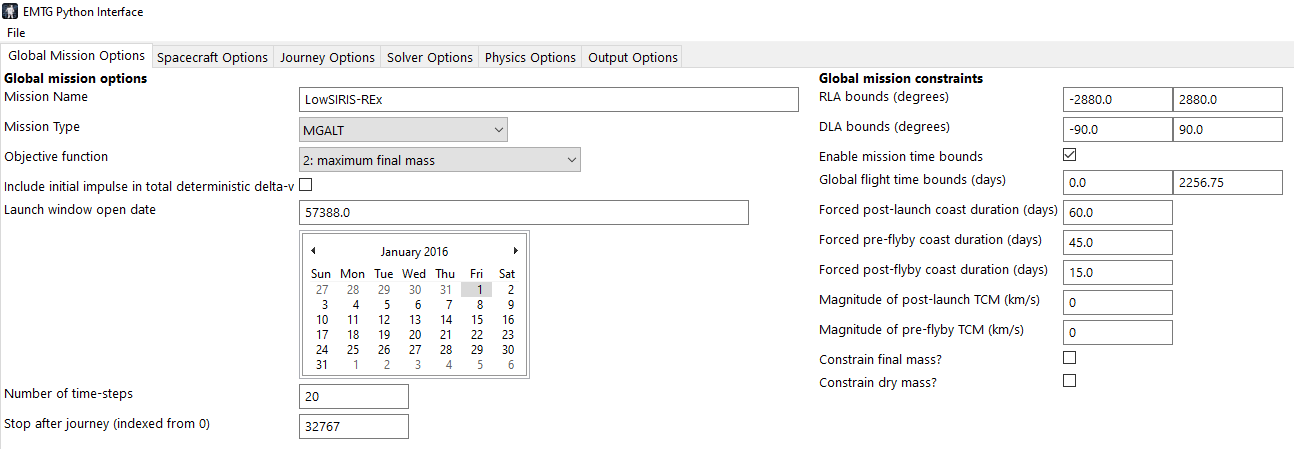
\includegraphics[width=\linewidth]{LowSIRIS-REx_global_options.png}}
	\caption{\label{fig:global_options}Global Options.}
\end{figure}

%%%%%%%%%%%%%%%%%%%%%
\subsection{Spacecraft Options}
\label{sec:spacecraft_options}
%%%%%%%%%%%%%%%%%%%%%

Switch to the ``Spacecraft Options'' tab and set the following options as shown in Figure \ref{fig:spacecraft_options}:

\begin{itemize}
	\item \textbf{Allow initial mass to vary:} ``On''
	\begin{itemize}
		\item Lets \ac{EMTG} use less initial mass than the launch vehicle can inject to a given C3 if that results in a higher final mass. Even with this checked, \ac{EMTG} will not allow the initial mass to be greater than the capabilities of the launch vehicle. 
	\end{itemize}
	\item \textbf{Power margin (fraction):} ``0.15''
	\begin{itemize}
		\item This effectively decreases the power made available to the propulsion system, compared to what is theoretically available.
	\end{itemize}
	\item \textbf{Thruster duty cycle:} ``0.9''
	\begin{itemize}
		\item This is a multiplier on the calculated thrust acceleration and is used to approximately take into account the fact that low-thrust spacecraft must periodically coast to allow for activities like navigation to take place. Both this setting and that for the previous option are standard for \acs{NASA} preliminary design.
	\end{itemize}
	\item \textbf{Power and Propulsion Coefficients:} Use Table \ref{tab:power_propulsion_coefs}

\end{itemize}

\begin{figure}[H]
	\centering
	\fbox{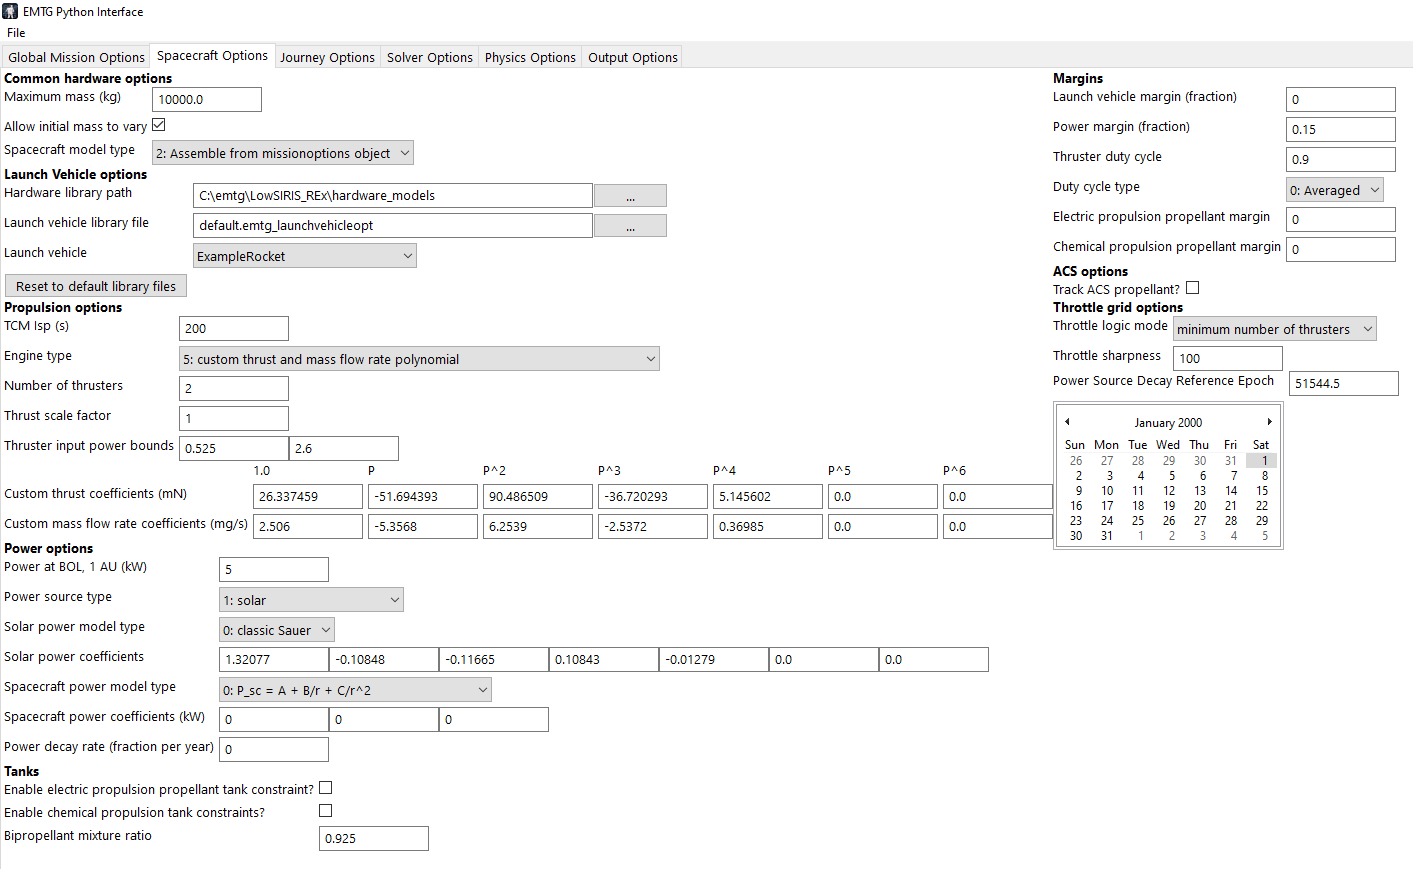
\includegraphics[width=\linewidth]{LowSIRIS-REx_spacecraft_options.png}}
	\caption{\label{fig:spacecraft_options}LowSIRIS-REx Thruster Settings.}
\end{figure}


\begin{table}[H]
	\begin{small}
		\begin{tabularx}{\linewidth} { >{\centering\arraybackslash} X >{\centering\arraybackslash} X >{\centering\arraybackslash}X >{\centering\arraybackslash}X  >{\centering\arraybackslash}X  >{\centering\arraybackslash}X   }
 			\hline
 			Parameter & 1.0 & P & P2 & P3 & P4 \\
			\hline 
 			Custom thrust coefficient (mN) & 26.337459 & -51.694393 & 90.486509 & -36.720293 & 5.145602 \\ 
 			Custom mass flow rate coefficients (mg/s) & 2.506 & -5.3568 & 6.2539 & -2.5372 & 0.36985 \\ 
 			\hline
		\end{tabularx}
	\end{small}
	\caption{\label{tab:power_propulsion_coefs}Spacecraft Propulsion Coefficients.}
\end{table}


%%%%%%%%%%%%%%%%%%%%%
\subsection{Journey Options}
\label{sec:journey_options}
%%%%%%%%%%%%%%%%%%%%%

Switch to the ``Journey Options'' tab and, starting with the ``Earth\_to\_Bennu'' Journey, set the following options as shown in Figure \ref{fig:earth_to_bennu_journey_options}:

\begin{itemize}
	\item \textbf{Journey arrival type:} ``3: rendezvous (no maneuver)''
	\begin{itemize}
		\item This means that the spacecraft is not allowed to perform an impulse at arrival (because it does not have a chemical engine). Instead, the low-thrust propulsion system will be required to gradually change the speed of the spacecraft to match the position and velocity of Bennu at arrival.
	\end{itemize}
	\item \textbf{Flyby sequence} ``[]''
	\begin{itemize}
		\item For LowSIRIS-REx, the Earth flyby should be removed because it is less optimal than a direct-to-Bennu trajectory.
	\end{itemize}
\end{itemize}

\begin{figure}
	\centering
	\fbox{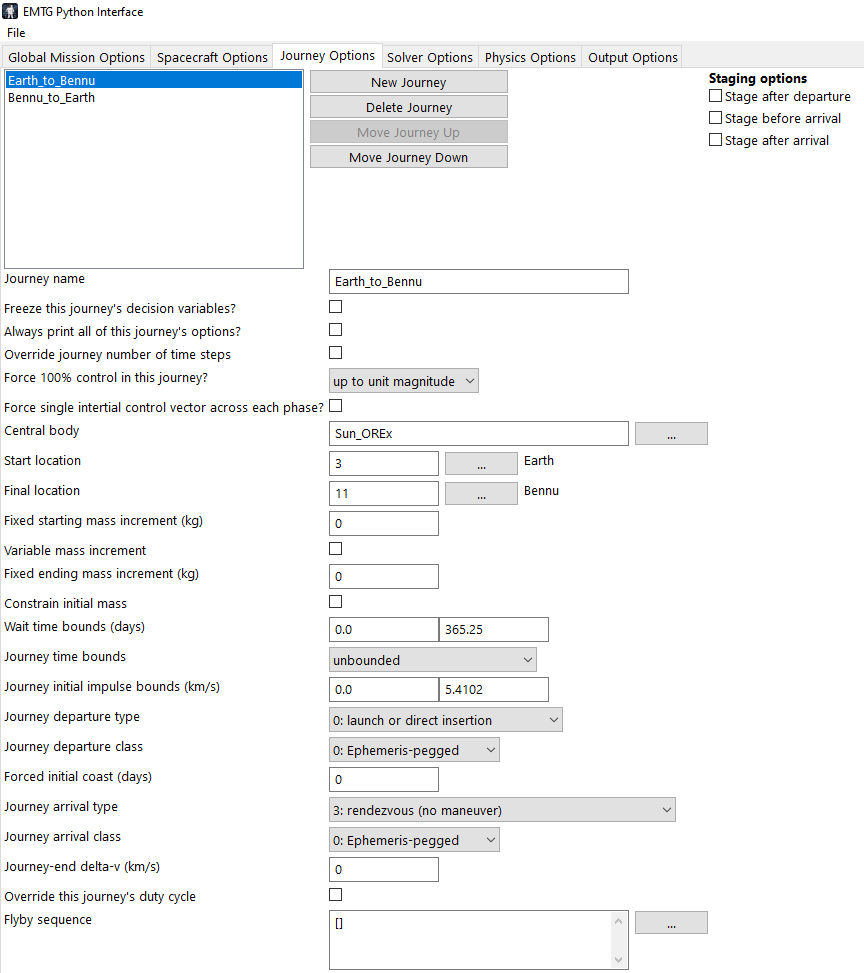
\includegraphics[width=\linewidth]{LowSIRIS-REx_earth_to_bennu_journey_options.png}}
	\caption{\label{fig:earth_to_bennu_journey_options}Earth to Bennu Journey.}
\end{figure}

\noindent Switch to the ``Bennu\_to\_Earth'' Journey and make the following changes as shown in Figure \ref{fig:bennu_to_earth_journey_options}:

\begin{itemize}
	\item \textbf{Departure type:} ``2: free direct departure''
	\begin{itemize}
		\item This means that the spacecraft starts with the position and velocity of Bennu and no initial impulse.
	\end{itemize}
	\item \textbf{Forced terminal cost (days:} ``90'' days
	\begin{itemize}
		\item This means that no thrust is allowed 90 days prior to Earth return. The spacecraft can make small adjustments using chemical thrusters during that time, but the electric propulsion system will not be used. (The small adjustments with chemical maneuvers are statistical maneuvers and are not modeled in this tutorial.)
	\end{itemize}
\end{itemize}

\begin{figure}[H]
	\centering
	\fbox{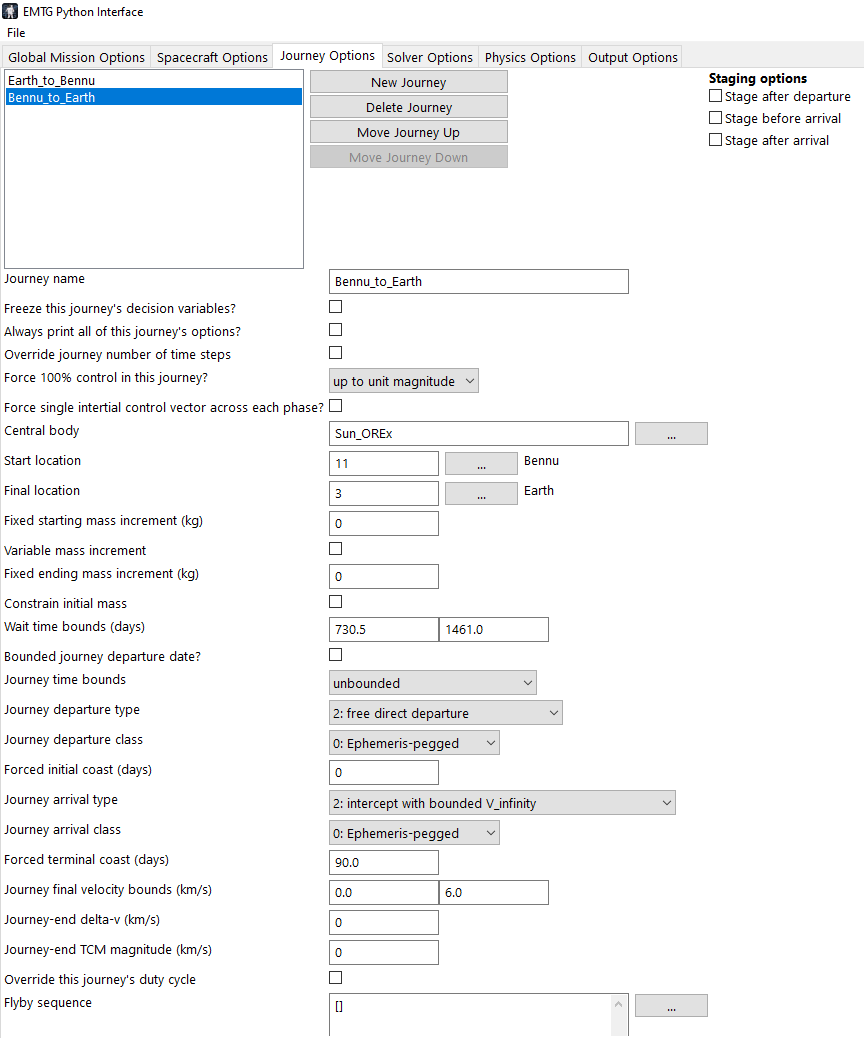
\includegraphics[width=\linewidth]{LowSIRIS-REx_bennu_to_earth_journey_options.png}}
	\caption{\label{fig:bennu_to_earth_journey_options}Bennu to Earth Journey.}
\end{figure}

%%%%%%%%%%%%%%%%%%%%%
\subsection{Solver Options}
\label{sec:solver_options}
%%%%%%%%%%%%%%%%%%%%%

No changes are needed to the Solver options here. However, you may want to increase “Maximum run time (s)” from the default 60 to, say, 120, if \ac{EMTG} does not find a feasible solution using the default value. In general, a low-thrust mission requires more time to find feasible and optimal solutions than a chemical mission because the optimization problem is larger: more decision variables and more constraints. The Solver options can be seen in Figure \ref{fig:solver_options}.

\begin{figure}[H]
	\centering
	\fbox{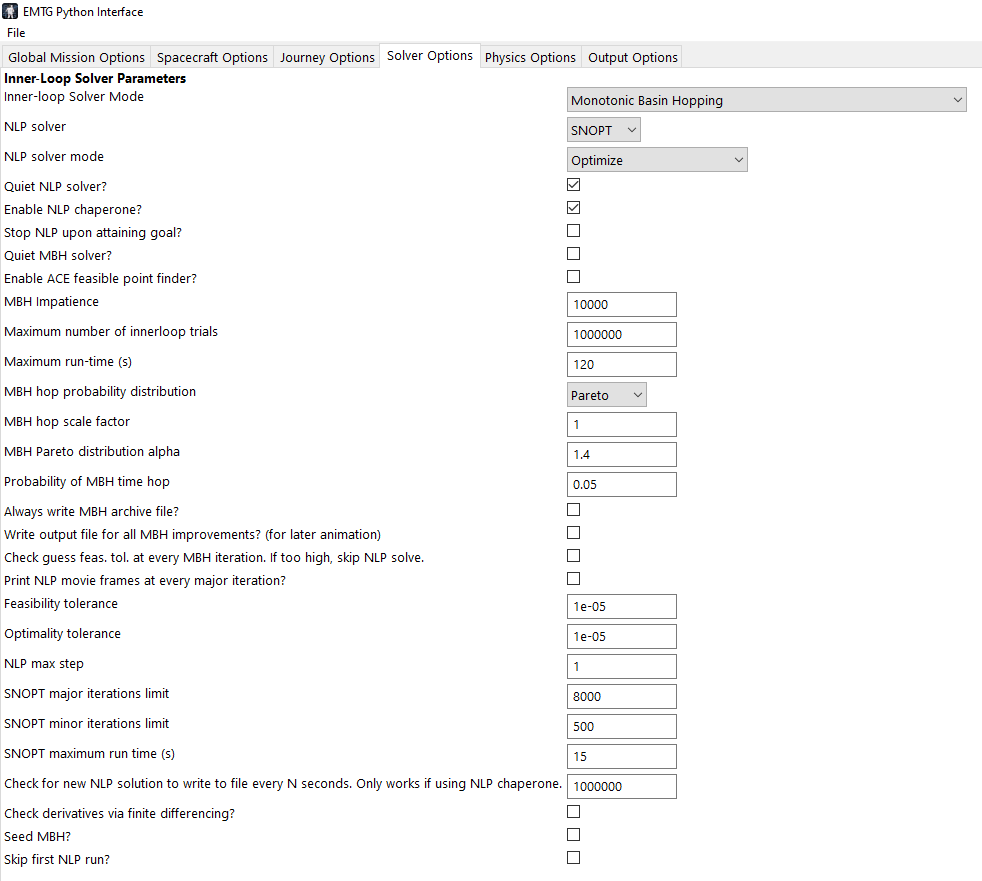
\includegraphics[width=\linewidth]{LowSIRIS-REx_solver_options.png}}
	\caption{\label{fig:solver_options}Solver Options.}
\end{figure}

%%%%%%%%%%%%%%%%%%%%%
\section{Run and Post-Process}
\label{sec:run_and_post_process}
%%%%%%%%%%%%%%%%%%%%%

Run the mission (File-\textgreater Run or Ctrl+r) and plot the trajectory when finished. Keep in mind that the maximum run time is short, and solutions may vary from run to run due to the stochastic nature of monotonic basin hopping. An example plot can be seen in Figure \ref{fig:traj_plot}.

\begin{figure}[H]
	\centering
	\fbox{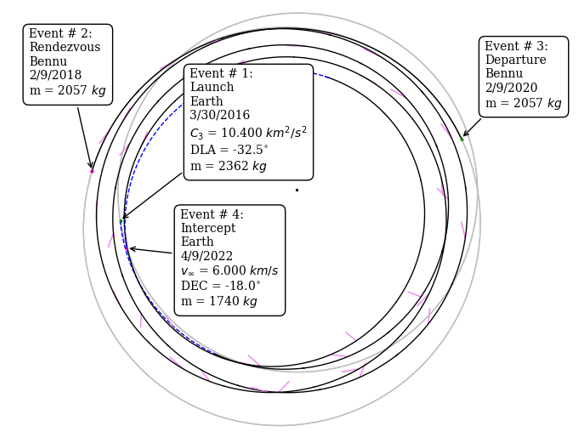
\includegraphics[width=\linewidth]{LowSIRIS-REx_trajectory_plot.png}}
	\caption{\label{fig:traj_plot}Trajectory Plot.}
\end{figure}

\noindent In addition to trajectory plots, PyEMTG can create plots of systems parameters, such as power, propulsion, and distance from the Sun and Earth. PyEMTG can also map the continuous low-thrust model to a discrete throttle table if you have one. An example data plot can be seen in Figure \ref{fig:example_data_plot}. 

\noindent \knownissuelabel{Note: Keep in mind that some options, such as ``Distance from Earth'' will not work without installing additional python packages.}{plotting_python_packages_issue}

\begin{figure}[H]
	\centering
	\fbox{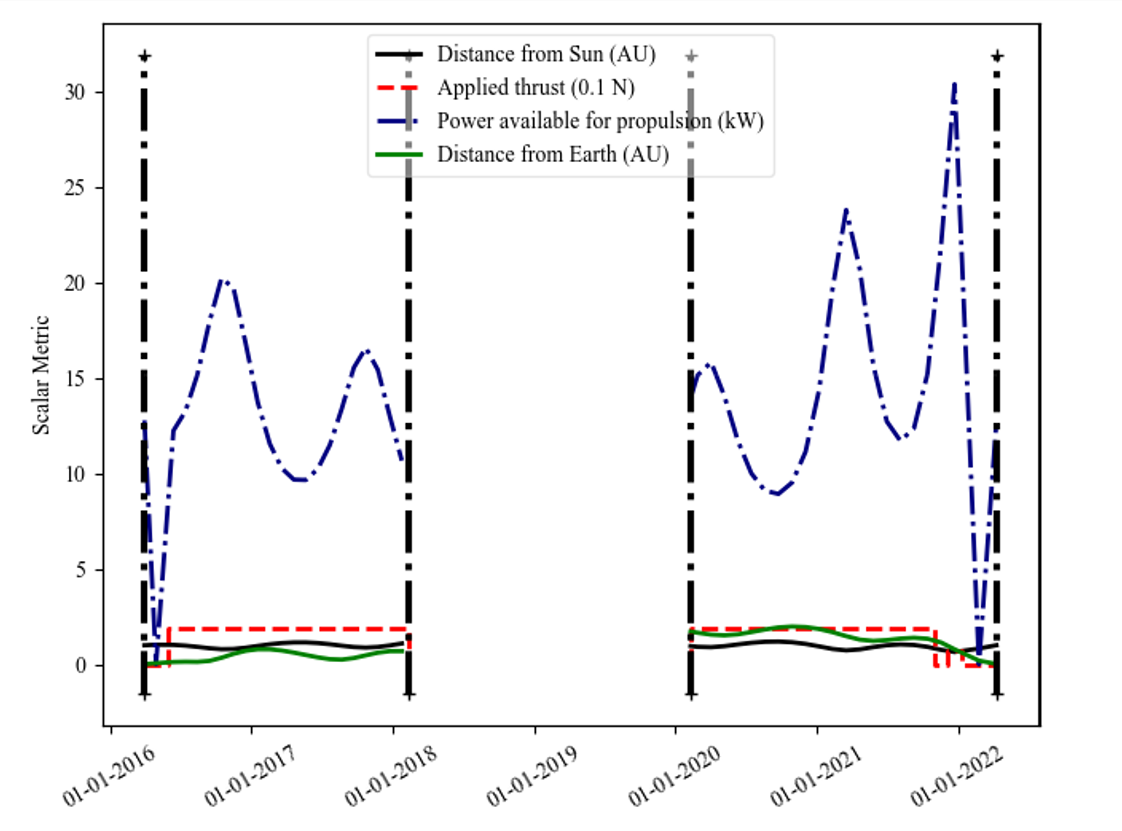
\includegraphics[width=\linewidth]{LowSIRIS-REx_data_plot.png}}
	\caption{\label{fig:example_data_plot}Example Data Plot.}
\end{figure}

%%%%%%%%%%%%%%%%%%%%%
\section{LowSIRIS-REx Medium-High Fidelity Options}
\label{sec:LowSIRIS-REX_med_high_fidelity}
%%%%%%%%%%%%%%%%%%%%%

The \ac{MGALT} transcription is not adequate for detailed design work because it approximates the true low-thrust trajectory with a sequence of conic arcs and bounded impulses (the Sims-Flanagan model). For a more accurate representation of the trajectory,  the \ac{FBLT} transcription will be used, which utilizes a numerical integrator and the true low-thrust equations of motion. \ac{FBLT} can support perturbing accelerations like third-body gravity and \ac{SRP}. (This is optional and these perturbations will not be turned on in this example.) However, only changing the transcription from \ac{MGALT} to \ac{FBLT} does not change the body encounters from patched-conic to “real” encounters. \ac{EMTG} does support fully integrated gravity assists, orbit insertion, escape, etc., but these are outside the scope of this tutorial.

%%%%%%%%%%%%%%%%%%%%%
\subsection{Global Options}
\label{sec:med_high_fidelity_global_options}
%%%%%%%%%%%%%%%%%%%%%

Change the following options in the ``Global Mission Options'' tab as shown in Figure \ref{fig:med_high_fidelity_global_options}:

\begin{itemize}
	\item \textbf{Mission name:} ``LowSIRIS-REx\_FBLT.emtgopt''
	\begin{itemize}
		\item Perform File-\textgreater Save (Ctrl+s) and make sure that the save file name and location are correct.
	\end{itemize}
	\item \textbf{Mission type:} ``\ac{FBLT}''
	\item \textbf{Number of time-steps:} ``40''
	\begin{itemize}
		\item A higher resolution trajectory is needed, i.e., more opportunities to change the control. If using as an initial guess a previous EMTG solution with a different number of time steps, EMTG will automatically interpolate the initial guess.
	\end{itemize}
\end{itemize}

\begin{figure}[H]
	\centering
	\fbox{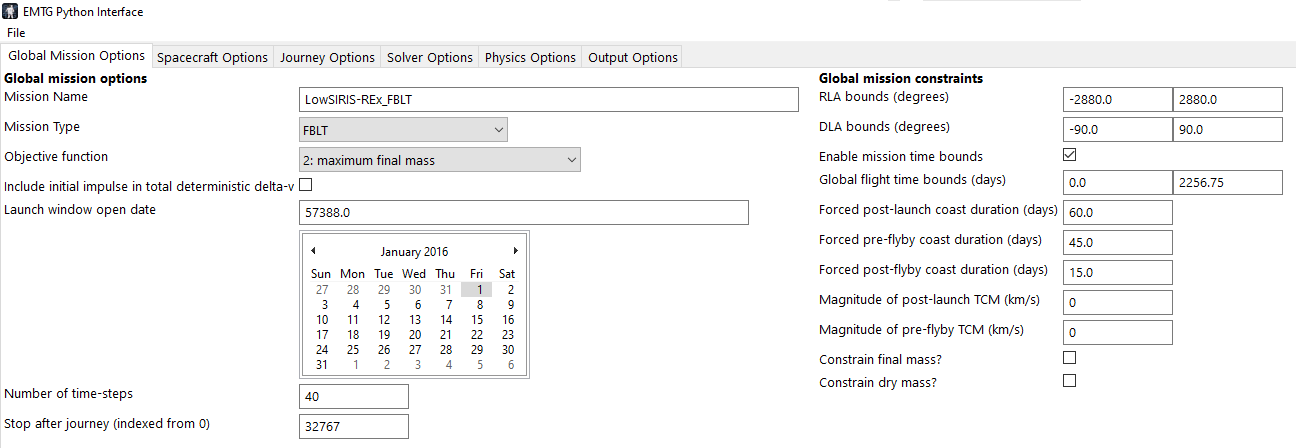
\includegraphics[width=\linewidth]{LowSIRIS-REx_med_high_fidelity_global_options.png}}
	\caption{\label{fig:med_high_fidelity_global_options}LowSIRIS-REx \ac{FBLT} Global Mission Options.}
\end{figure}

%%%%%%%%%%%%%%%%%%%%%
\subsection{Solver Options}
\label{sec:med_high_fidelity_solver_options}
%%%%%%%%%%%%%%%%%%%%%

Switch to the “Solver Options” tab and change the following options as shown in Figure \ref{fig:med_high_fidelity_solver_options}:

\begin{itemize}
	\item \textbf{Inner-loop Solver Mode:} ``\acs{NLP} with initial guess''
	\begin{itemize}
		\item Since there is a solution in \ac{MGALT}, \ac{MBH} does not need to be run. Instead, only the \ac{NLP} solver \acs{SNOPT} will be run, using the \ac{MGALT} solution as an initial guess.
	\end{itemize}
	\item \textbf{Quiet \ac{NLP} solver:} ``Off''
	\begin{itemize}
		\item Uncheck this option so you can see \acs{SNOPT} iterate.
	\end{itemize}
	\item \textbf{\acs{SNOPT} maximum run time (s):} ``600'' seconds
	\begin{itemize}
		\item \ac{FBLT} is very slow because of the numerical integration of the equations of motion, as compared to \ac{MGALT}'s Kepler problem solves, so let’s give \acs{SNOPT} 10 minutes to chew on the problem.
	\end{itemize}
\end{itemize}

\begin{figure}[H]
	\centering
	\fbox{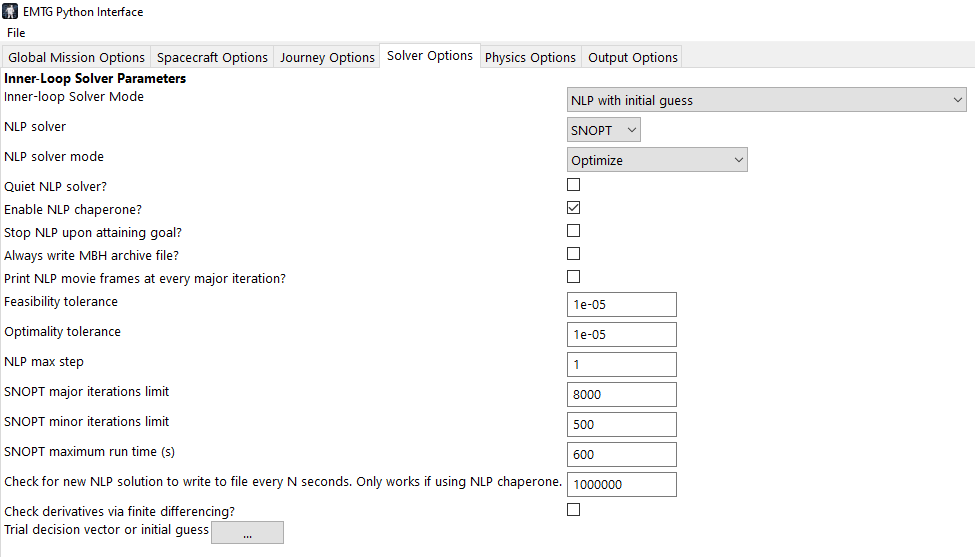
\includegraphics[width=\linewidth]{LowSIRIS-REx_med_high_fidelity_solver_options.png}}
	\caption{\label{fig:med_high_fidelity_solver_options}\ac{FBLT} Solver Options.}
\end{figure}

%%%%%%%%%%%%%%%%%%%%%
\subsection{Physics Options}
\label{sec:med_high_fidelity_physics_options}
%%%%%%%%%%%%%%%%%%%%%

Switch to the ``Physics Options'' tab and set the following options:

\begin{itemize}
	\item \textbf{Integrator type:} ``rk8 fixed step''
\end{itemize}

\noindent The default integrator time step of 86400 seconds is appropriate for this run.

\noindent \knownissuelabel{Note: The “rk7813M adaptive step” option does not work.}{broken_integrator_issue} 

%%%%%%%%%%%%%%%%%%%%%
\section{Run and Post-Process}
\label{sec:med_high_fidelity_run_and_post_process}
%%%%%%%%%%%%%%%%%%%%%

Run the mission as before. This time the \acs{SNOPT} output will be displayed to the terminal. After the \ac{EMTG} run finishes, plot the journeys and experiment with some of the Data Plots. If you examine the .emtg solution files in a text editor, you’ll see that the journeys are represented by more data points than before due to the increased number of time-steps set in Global Options. Figure \ref{fig:med_high_fidelity_traj_plot} shows an example trajectory plot, while Figure \ref{fig:med_high_fidelity_data_plot} shows an example Data Plot.

\noindent You now know how to use \ac{EMTG} to refine an initial \ac{MGALT} solution into a higher-fidelity \ac{FBLT} solution. Additional steps to creating a ``real'' trajectory include turning on non-two-body forces and explicitly modeling launch, flybys, and arrival, but these are outside the scope of this tutorial.

\begin{figure}[H]
	\centering
	\fbox{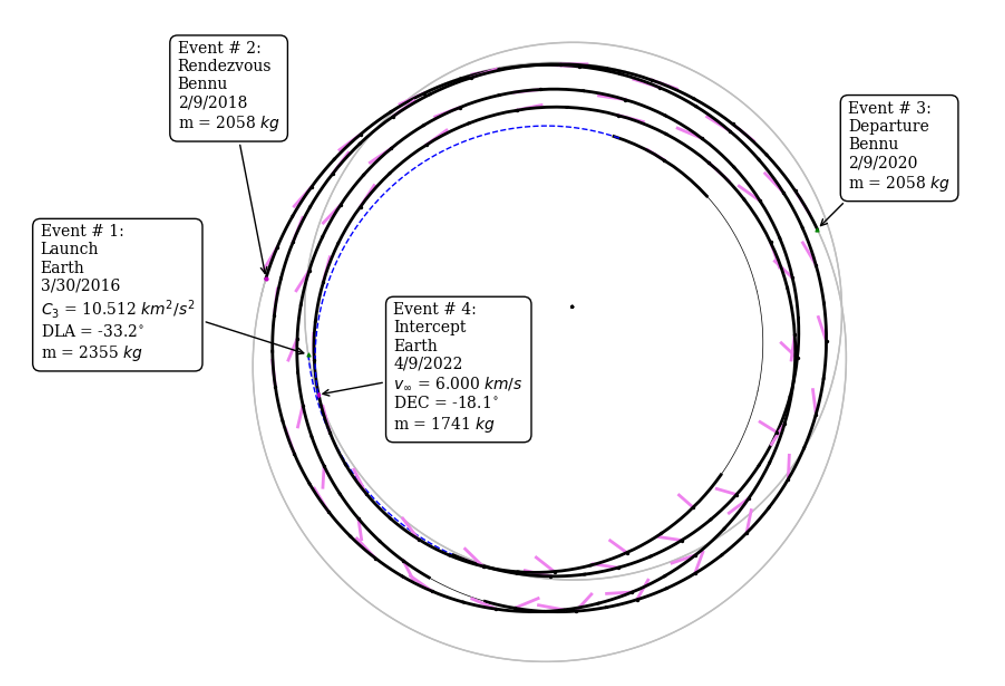
\includegraphics[width=\linewidth]{LowSIRIS-REx_med_high_fidelity_trajectory_plot.png}}
	\caption{\label{fig:med_high_fidelity_traj_plot}\ac{FBLT} Example Solution.}
\end{figure}

\begin{figure}[H]
	\centering
	\fbox{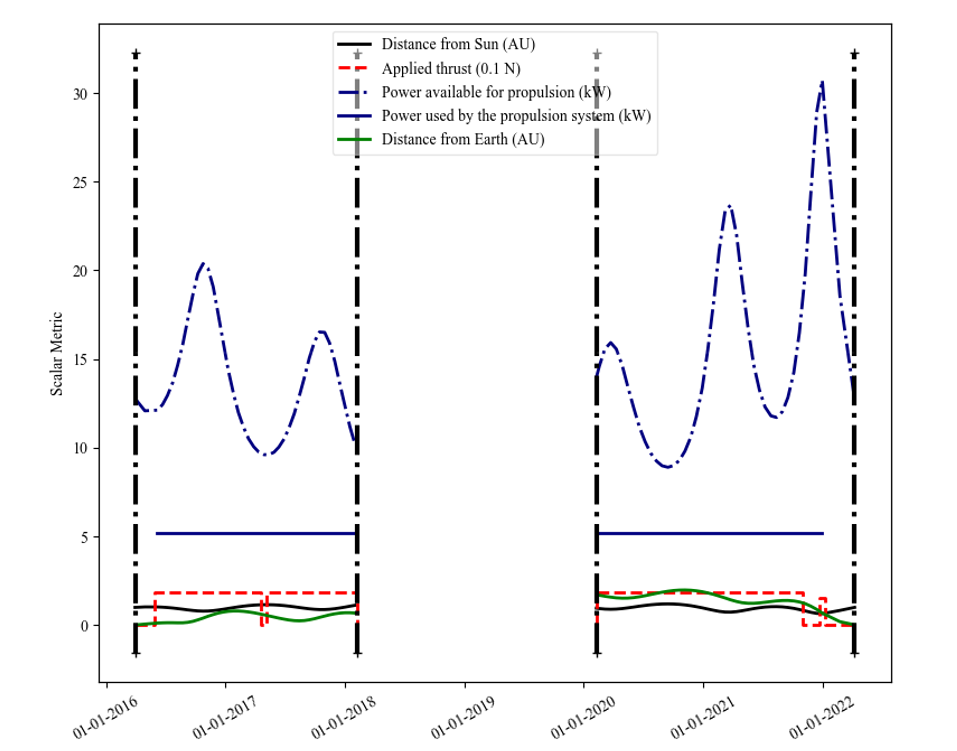
\includegraphics[width=\linewidth]{LowSIRIS-REx_med_high_fidelity_data_plot.png}}
	\caption{\label{fig:med_high_fidelity_data_plot}\ac{FBLT} Example Data Plot.}
\end{figure}


\end{document}